\documentclass{article}
\usepackage{imakeidx}
\usepackage{graphicx}
\usepackage{wrapfig}
\usepackage{mathtools}
\graphicspath{{images/}}
\usepackage{geometry}
\geometry{a4paper,
total={170mm, 257mm},
left = 30mm,
right = 30mm,
bottom = 30mm,
top = 30mm
}

\usepackage{multicol}
\title{Computational Vision \linebreak Revision Notes}
\author{James Brown}
\makeindex
\begin{document}
	\pagenumbering{gobble}
	\maketitle
	\newpage
	\tableofcontents
	\newpage
	\pagenumbering{arabic}

	\section{Introduction}
	These are notes I have written in preparation of the 2017 Computation Vision exam. This year the module was run by Hamid Deghani (H.Dehghani@cs.bham.ac.uk).
	\linebreak \linebreak
	Computational vision is the acquisition of knowledge about objects and events in the environment through information processing of light emitted or reflected from objects. In short - we want to make a computer know what is where, by looking through information. We can also use computational vision to do automatic inference of properties of the world from images.

	\section{Human Vision}
	\par
	As humans we have evolved eyes which perceive the visible section of the electromagnetic spectrum, which falls between the wavelengths of 380nm - 760nm. Red light lies at the longer end (760nm) of visible light, and purple at the shorter end (380nm). \index{visible light}Visible light is strongly absorbed in the human eye because it can cause an electron to jump to a higher energy levels - yet it does not have enough energy to ionize cells. The evolutionary process of evolving eyes began more than 3 billion years ago with the formation of photopigments. These are molecules where light incident upon them will trigger a physical or chemical change. \index{photopigment}Photopigments capture photons which lead to the release of energy in the photopigment. This is may be used for photosynthesis or a behavioural reaction (a nerve reaction). A single \index{photocell}photocell contains multiple layers to catch light, not just one. This increases the chance of catching any one individual photon - if it's not caught by the first layer it's much more likely to be caught by the second and so on.

	\subsection{Image Formation}
	Photocells contain a light sensitive patch of photopigments. Using a single cell we can capture light in 1 dimension, but we can't really 'see'. All we can do is tell if the light is on, or off. With multiple cells we can have better direction resolution and with multiple cells we have a very wide aperture - we can't tell exactly where the image is. The image formed will be very bright but extremely fuzzy. This became curved over time and this which really helped with direction resolution as light incident on the left side of the curve must have come from the right. Images formed this way are still very blurry and will result in multiple projections of the same image. Over time eyes evolved to become \index{pinhole camera}pinhole cameras which form sharp yet dim images by allowing light to come from a single source (the pinhole) - effectively throwing away loads of potential information about the image. The solution to form sharp and bright images was to use a \index{lens}lens at the front of the eye. The lens focuses all incoming light to a single point and from there we can use our simple pinhole camera for forming images. It should be noted that the image formed is upside down to what exists in reality.
	
	\subsection{Retina Processing}
	The human \index{retina}retina contains two kinds of \index{photoreceptors}photoreceptors which respond to incident light - \index{rods}\textbf{rods}  (around 120 million) and \index{cones}\textbf{cones} (around 6 million). Rods are extremely sensitive photosensors and respond to a single photon of light. Multiple rod cells converge to the same \index{ganglion cell}ganglion cell and therefore neuron within the \index{retina} which results in poor spatial resolution. Rods are responsible simply for detecting the presence of light, and as a result make up the entirety of our night-vision. On the other hand, cones are active at much higher light levels and responsible for the detection of different colours of light. Cones have a much higher resolution as they are processed by several different neurons. Within the eye we have a \index{receptive field}receptive field, which is the area on which light must fall for a neuron to be stimulated. It should be noted that receptive field in the center of the eye is much smaller than it is for the periphery of the eye.
	
	\subsection{The Visual Pathway}
	Vision is generated by photoreceptors in the retina. All the information captured leaves the eye by way of the optic nerve\index{optic nerve}. There is a partial crossing of axons at the optic chiasm\index{chiasm}. This is only partial as information from both eyes is sent to both sides of the brain - this allows us to process depth. After this chiasm, the axons are called the optic tract. The optic tract wraps around the midbrain to get to the lateral geniculate nucleus (LGN)\index{lateral geniculate nucleus}. The LGN axons fan out through the deep white matter of the brain and ultimately to the visual cortex\index{visual cortex}.
	\begin{figure}[h]
		\centering
		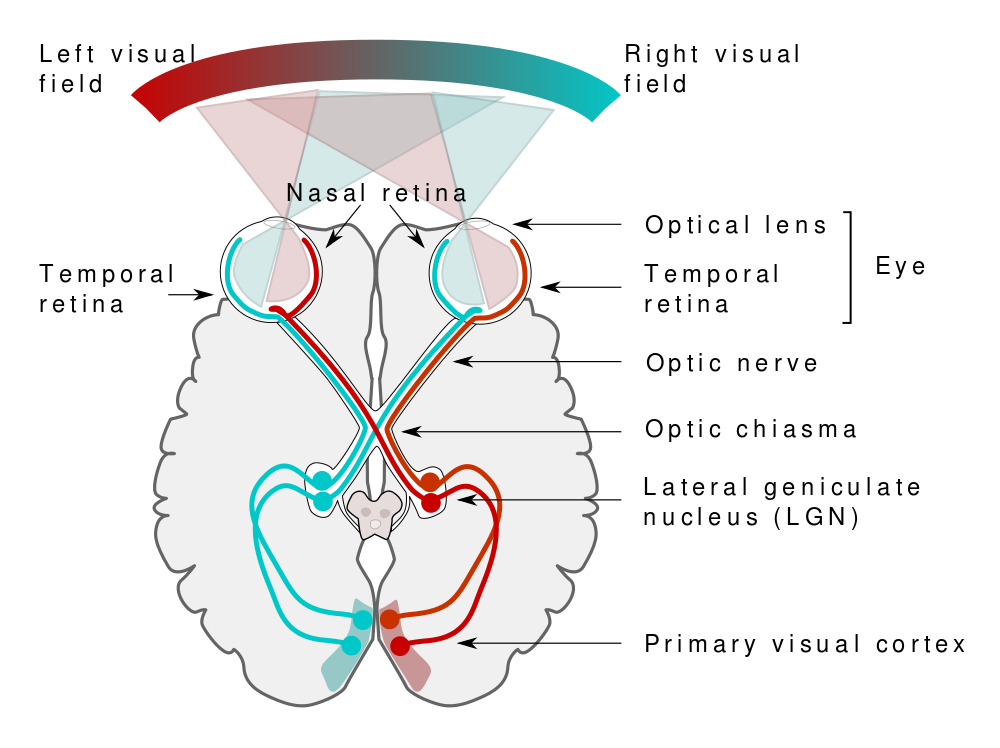
\includegraphics[width=0.6\textwidth]{visual_pathway}
		\caption{The visual pathway in the human brain}
		\label{fig:visual pathway}
	\end{figure}
	
	\subsection{Colour Processing}
	Objects in the world selectively absorb some wavelengths (a colour) and reflect other wavelengths. Human retinas contain three different types of cones to respond to different colours. This gives us the ability to distinguish different forms of the same object - for example: unripe, ripe and off fruit. Many theories of colour vision have been proposed and some have been hard to disprove until recently. 
	\par	
	In 1802 Young proposed that the eye has three different types of receptors, each of which are sensitive to a single hue. From this he proposed that any colour can be produced by appropriate mixing of the three primary colours. This is known as the trichromatic theory\index{trichromatic theory}.
	
	\par 
	Hering suggested that colour may be represented in a visual system as 'opponent colours' in the 1930's.
	
	
	\section{Edge Detection}
	\subsection{Intensity Images}
	An intensity image\index{intensity image} is a data matrix whose values represent intensities within some range. Each element of the matrix corresponds to one image pixel\index{pixel}. An indexed image consists of a data matrix, $X$, and a colour map\index{colour map} matrix, $map$. $map$ is a $m$-by-3 array of double containing floating point values in the range $[0, 1]$. Each row in the map specifies the red, green an blue components of a single color. Each cell in the indexed image then specifies the corresponding colour from the colour map. In an intensity image can be thought of as a function $f(x, y)$ mapping coordinates to intensity. From this we can calculate an intensity gradient\index{intensity gradient}.
	\begingroup
	\renewcommand*{\arraystretch}{1.5}
	\[ \overrightarrow{G}[f(x,y)] = \begin{bmatrix}G_{x} \\ G_{y} \end{bmatrix} = \begin{bmatrix} \frac{df}{dx} \\ \frac{df}{dy} \end{bmatrix} \]	
	\endgroup

	 This is a vector which we can think of as having an $x$ and $y$ component. We can calculate both the magnitude and direction for this gradient of intensity. 
	\begin{multicols}{2}
		\noindent
		\centering
			$M(\overrightarrow{G}) = \sqrt{G_{x}^{2} + G_{y}^{2}}$ \\
			$\alpha(x, y) = \tan^{-1}\left(\frac{G_y}{G_x}\right)$
	\end{multicols}
	
	When calculating the magnitude, figuring out a square root can be very computationally expensive. It's possible to replace this with an approximation: $M(\overrightarrow{G}) = |G_{x}| + |G_{y}|$
	
	\subsection{Approximating the Intensity Gradient}
	In order to approximate the gradient we may use a variety of different masks over the image, such as the Roberts and Sobel detectors. These masks use the idea of convolution in order to calculate the rate of change of intensity at each pixel. Convolution is the computation of weighted sums of image pixels. For each pixel in the image, the new value is calculated by translating the mask to the pixel and taking the weighted sum of all the pixels in the neighbourhood. Once we have a value for the rate of change of the intensity gradient we can threshold our image to produce the locations of edges.
	
	\section{Noise Filtering}
	When taking images we also gather a lot of noise which results in fake edges once we apply our edge detectors. We would like to remove this noise and we many filters which can be implemented by the idea of convolution. The most widely used of these filters is the Gaussian filter\index{gaussian filter}, although there are other simpler filters such as the mean filter\index{mean filter}.
	\begin{figure}[ht]
	\begin{minipage}{.5\textwidth}
			\begingroup
			\renewcommand*{\arraystretch}{1.7}	
			\centering
			\[ \begin{bmatrix} \frac{1}{9} & \frac{1}{9} & \frac{1}{9} \\
								\frac{1}{9} & \frac{1}{9} & \frac{1}{9} \\
								\frac{1}{9} & \frac{1}{9} & \frac{1}{9}
			\end{bmatrix} \]
			\endgroup
			\caption{An example mean filter}
			\label{fig:mean filter}
	\end{minipage}
	\begin{minipage}{.5\textwidth}
		\centering
		\[ \begin{bmatrix} 0 & .01 & .02 & .01 & 0 \\
								.01 & .06 & .11 & .06 & .01 \\ 
							    .02 & .11 & .16 & .11 & .02 \\
							    .01 & .06 & .11 & .06 & .01 \\
							    0 & .01 & .02 & .01 & 0
				\end{bmatrix} \]
		\caption{An example Gaussian filter}
		\label{fig:gaussian filter}

	\end{minipage}
	\end{figure}
	
	The mean filter averages a pixels value with all of the surrounding intensities for a new value. A Gaussian filter follows the same principle as this but uses a weighting, valuing pixels closer to the original more than pixels farther away.	The Gaussian filter has an extra bonus of being able to be applied as two individual 1D Gaussian filters in sequence rather than one large 2D filter as shown below.
	\begin{figure}[ht]
	\begin{multicols}{2}
		\[\begin{bmatrix} 0.0545 & 0.2442 & 0.4026 & 0.2442 & 0.0545 \end{bmatrix} \] \\
		\[\begin{bmatrix} 0.0545 \\ 0.2442 \\ 0.4026 \\ 0.2442 \\ 0.0545 \end{bmatrix} \]
	\end{multicols}
	\caption{A Gaussian filter deconstructed to two 1D filters which can be applied in sequence}
	\label{fig:1d gaussian filter}
	\end{figure}
	
	\section{Advanced Edge Detection}
	Intensity changes can be caused by geometric events such as surface orientation discontinuities, depth discontinuities, color discontinuities and texture discontinuities. It can also be caused by non-geometric events such as illumination changes, specularities, shadows and inter-reflections. All of these events can be used to try to find edges in the image. When we try to detect edges, we are trying to produce a line 'drawing' of a scene from an image of that scene. We use this to extract important features of an image, such as corners and curves. These features are then used by higher-level computer vision algorithms.
	
	\subsection{Main steps in Edge Detection}
	Regardless of methods, there a few major steps to edge detection:
		\begin{enumerate}
			\item \textbf{Smoothing}: suppress as much noise as possible, without destroying any of the true edges.
			\item \textbf{Enhancement}: apply differentiation to enhance the quality of edges (i.e. sharpening).
			\item \textbf{Thresholding}: determine which edge pixels should be discarded as  noise and which should be retained (i.e. threshold edge magnitude).
			
			\item \textbf{Localization}: determine the exact edge location.
		\end{enumerate}

	\par
	Most of the time, points that lie on an edge are detected by 
		\begin{enumerate}
			\item Detecting the local \textit{maxima} or \textit{minima} of the first derivative.
			\item Detecting the \textit{zero-crossings}\index{zero crossing} of the second derivative
		\end{enumerate}
		
	There are a few practical issues that come with this. When smoothing an image, the smoothing effect achieved depends on the mask size (for example, with a Gaussian filter it depends on $\sigma$). A larger mask will reduce noise more, but it also worsens localization and adds uncertainty to the location of the edge.
	
	Based on this we can draw up some criteria for an optimal method of edge detection:
	\begin{enumerate}
		\item \textbf{Good detection}: Minimize the probability of false positives and false negatives (spurious edges and missing real egdes).
		\item \textbf{Good localization}\index{localization}: Detected edges must be as close as possible to the true edges.
		\item \textbf{Single response}\index{single response}: Minimise the number of local maxima around the true edge.
	\end{enumerate}

	Canny showed that the first derivative of Gaussian closely approximates the operator that optimizes the product of signal-to-noise ratio\index{signal-to-noise ratio} and localization\index{localization}.

	\subsection{Hysteresis}
	Hysteresis thresholding\index{hysteresis thresholding} uses two thresholds - a low threshold $t_{l}$ and a high threshold $t_{h}$ (usually this is $2t_{l}$). This makes the assumption that important edges should be along continuous curves in the image. It allows us to follow a faint section of a given line and to discard a few noisy pixels that do not constitute a line but have produced large gradients. We begin by applying the high threshold - this marks edges that we can be fairly sure that are genuine. Starting from these points, and using the directional information derived earlier, edges can be traced throughout the whole image. While tracing an edge, we apply the lower threshold, allowing us to trace faint sections of edges as long as we find a starting point. 

	\section{Hough Transform}
	So far we haven't actually found edge segments, just lots and lots of edge points. The Hough Transform\index{hough transform} is a common approach to finding parameterised line segments. Every straight line in an image can be described by an equation. Each edge point in an image, if considered in isolation, could lie on an infinite number of straight lines. In Hough Transform each edge point votes for every line it could be on, and the lines with the most votes win.

	\section{Scale Invariant Feature Transform}
	We can now detect features in images. The most basic feature is edges, but through the use of Hough transform\index{hough transform} we can also detect lines and even geometric shapes such as circles. We want to detect features for various reasons, such as object recognition\index{object recognition}, wide baseline matching\index{wide baseline matching} and tracking\index{tracking}. In order to do this we need to make sure our features are scale invariant. Good features should be robust to all sorts of nastiness that can occur between two different images. There are many different causes of invariance:
	\begin{itemize}
		\item Illumination
		\item Scale
		\item Rotation
		\item Affine transformation (scaling and streching)
		\item Full perspective
	\end{itemize}
	
	\subsection{Dealing with Illumination Invariance}
	The easiest way to do this is to normalise the image. This is done by creating a histogram of all intensity values within the image. We can then stretch the histogram to match others of the same image in different illuminations (other images with different illumination should still have the same shape of histogram, even in not the exact same histogram). This stretch can be achieved through simple linear normalization.
	
	\subsection{Dealing with Scale Invariance}
	 One way to ensure our image is scale invariant is by trying to scale it up and down, and see if a feature exists regardless of how much the image is scaled. There are two main methods to achieve this: Pyramids\index{pyramids} and Scale Space\index{scale space} (DOG method\index{DOG method}). 
	
	\par	 
	 In the pyramids method, we divide the width and height of the image by 2. We take the average of 4 pixels for each new pixel and repeat this process until the image is very small. We can then run our filters (edge detectors) over the image to check for the existence of certain features. If the feature still exists all the way down, we can say that the feature is scale invariant. On the other hand, the DOG (Difference of Gaussian) method is very similar to pyramids. Instead will fill the gaps with blurred images. This is like having a nice linear scaling without any expense. We take the features from the differences of the images, and if the feature is repeatably present in between Difference of Gaussians it is scale invariant and we should keep it.
	
	\subsection{Dealing with Rotational Invariance}
		We can deal with rotational invariance\index{rotational invariance} in much the same way as we deal with illumination invariance. We want to rotate all features to go in the same way in a determined manner. To do this, we take a histogram of all edge directions in the image and then rotate the image to the most dominant rotation (or possibly even the second most dominant if it's good enough).
		
	\section{Face Recognition}

	\section{Motion}

	\section{ROC Analysis}
	Receiver operating characteristic analysis provides us tools to select possibly optimal models and to discard suboptimal ones. In order to carry out ROC analysis we need to count the different kind of errors that are possible. When classifying if a pixel is an edge or not, there are 4 possible situations - \textbf{true positive} (predicted it was an edge and it was), \textbf{false positive} (predicted it was an edge and it wasn't), \textbf{false negative} (predicted it wasn't an edge and it actually was) and \textbf{true negative} (predicted it wasn't an edge and it wasn't).
	
Once classifying each pixel, we then count the total number of each label (TP, FP, TN, FN) over the large dataset. In ROC analysis we use two statistics:
	\begin{multicols}{2}
		\noindent
		\centering
			$ \text{Sensitivity} = \frac{TP}{TP+FN}$ \\
			$ \text{Specificity} = \frac{TN}{TN+FP}$
	\end{multicols}	
	Sensitivity is the likelihood of spotting a positive case when presented with one or the proportion of edges we find. Specificity is the likelihood of spotting a negative case when presented with one or the proportion of non edges that we find. To define a ROC space we only need the true positive rate (TPR) and the false positive rate (FPR). The TPR is simply the sensitivity and the FPR is $1 - \text{specificity}$. We use the FPR and TPR as x and y axes respectively of the ROC space.
	
	\begin{wrapfigure}{r}{0.4\textwidth}
		\centering
		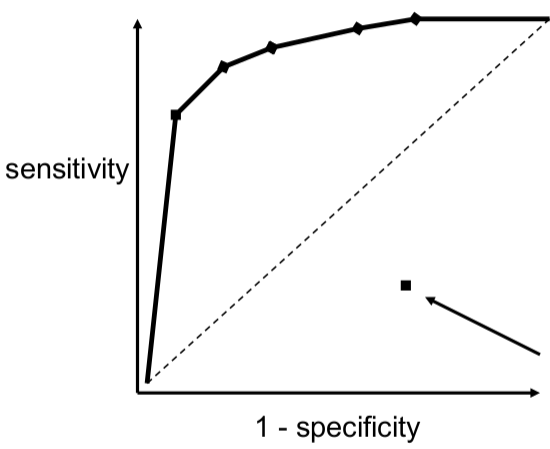
\includegraphics[width=0.4\textwidth]{roc_analysis}
		\caption{A sample ROC space}
		\label{fig:roc_analysis}
	\end{wrapfigure}
	
	All of the optimal detectors lie on the convex hull - the best possible position is for a detector to lie in the top left corner. It should be noted that if the edge detector lies below the dotted line then we can instantly make the detector better by simply just flipping the output of the algorithm!
		
	\section{Object Recognition}

	\section{Model Based Object Recognition}
	\newpage
	\listoffigures
	\printindex

\end{document}
